\documentclass[]{usiinfbachelorproject}
\usepackage{subfigure, wrapfig, url, array, caption,xcolor,amsmath,algorithm, tikz}
\usepackage{footnotebackref}
\usepackage[ngerman,english]{babel}
\usepackage[noend]{algpseudocode}
\newcommand\tab[1][1cm]{\hspace*{#1}}
\captionsetup{labelfont={bf}}

%%% For algorithms %%%
\makeatletter
\def\BState{\State\hskip-\ALG@thistlm}
\makeatother
%%%%%%%%%%%%%

\newcommand\transp[1]{{#1}^{\top}}

\author{Vanessa Braglia}

\title{The swiss scientific social network}
\versiondate{\today}

% DA SCOMMENTARE
%\begin{committee}
%\advisor[Universit\`a della Svizzera Italiana, Switzerland]{Prof.}{Olaf}{Schenk}
%\assistant[Universit\`a della Svizzera Italiana, Switzerland]{}{Fabio}{Verbosio}
%\end{committee}

\abstract {
In this project I implemented some algorithms to analyze the swiss scientific social network.
To construct the graph representing the relations (the edges) between authors (the nodes) I crawled some conferences' online programs and I have extracted all the necessary information. I used PageRank and graph partitioning to study the relationships between authors: I found the members that collaborate more with each other and the relationship between different institutions. The results provide an interesting picture of the different research scenarios in Switzerland and how they interact with each other internally to an establishment but also between different institutions. 
}


\begin{document}
% DA SCOMMENTARE
%\maketitle
\newpage
\tableofcontents
\newpage

%%%%%%%%%%%%%%%%%%%%%%%%%
\section{Introduction} \label{sec:intro} 
%%%%%%%%%%%%%%%%%%%%%%%%%

A social network consists of a set of objects connected to each other by social relations. The best way to model social networks is using graphs (see Figure \ref{fig:socialnetwork}): the objects (entities) are represented as nodes and the connections as edges between two different nodes. The most common example we can take is the World Wide Web (WWW) where we have web pages as nodes connected by hyperlinks, the edges.

\begin{figure}[ht]
	\centering
	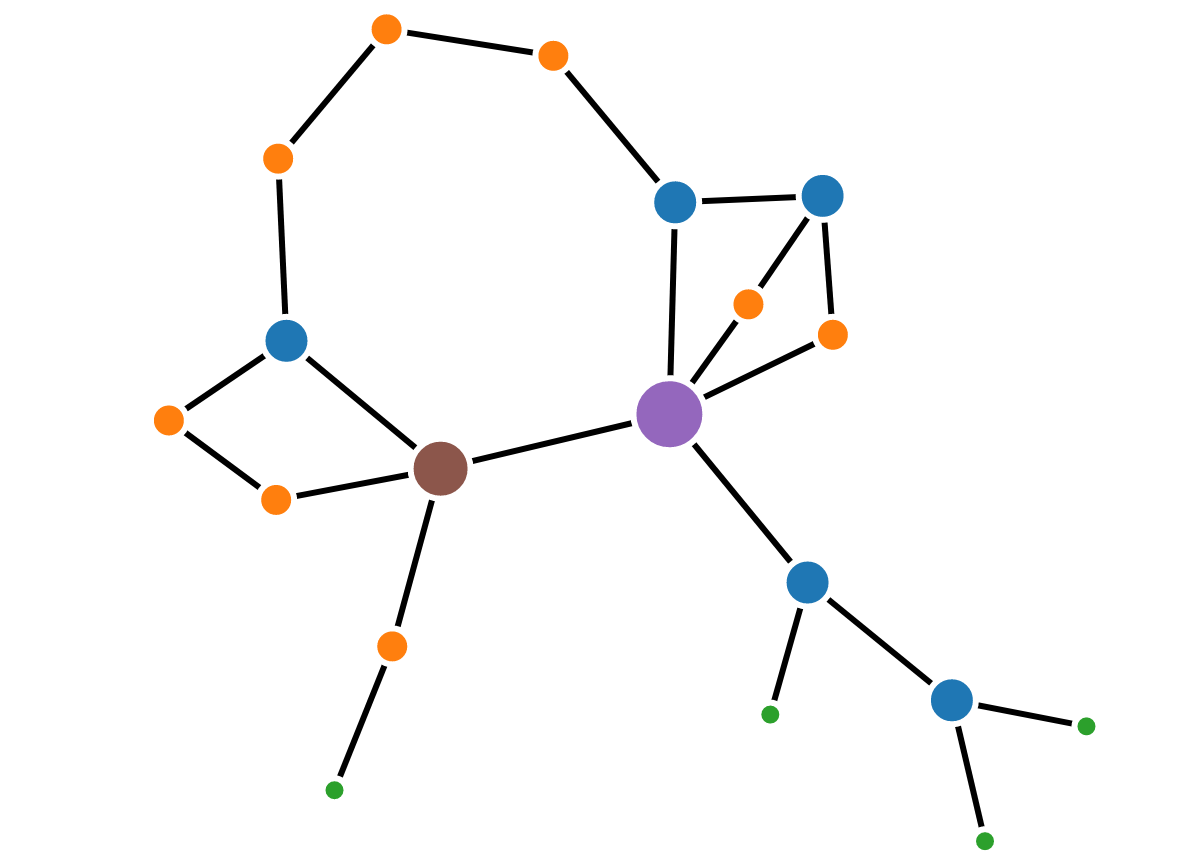
\includegraphics[height=4cm]{img/graph2.png}
	\caption{Example of social network graph}
	\label{fig:socialnetwork}
\end{figure}

The goal of this project is to create a social network of computational science authors belonging to Swiss institutions and then analyze the relative graph.

I want to find the relations between authors of the same or different institutions and belonging to the same or to different research scenarios: how they interact with each other and if they are strictly related to the institution or cooperate throughout Switzerland. The result will provide also a ranking of the authors and the institutions to see which are the most influential in the computational science research.

The first step is retrieving all the necessary information for the construction of the social network, i.e., names of the authors and relationships between each other. I crawled the 2015, 2016 and 2017 PASC Conferences and different SIAM conferences of several years, selecting the topics relevant to us (e.g. Optimization, Parallel Computing,...). The PASC conferences are interdisciplinary and bring together researchers across the areas of computational science, high-performance computing, and various domain sciences, 

The second step is the information analysis to find out relations between institutions and between members belonging to the same institution. With PageRank algorithm we obtain a ``ranking'' of all conferences' participants.
PageRank is an algorithm used by Google Search to rank websites in their search engine results, but it can be applied to any social network. In this project I use the algorithm to measure the importance of institutions' members considering the number and quality of their collaborations. I use graph partitioning techniques to invert the process and obtain the institutions from members collaborations: it is reasonable to assume that members of the same institution collaborate more between each other than with other institutions' representatives.

I also analyze the institutions' connectivity matrices and their structure: looking at the cliques present in the matrices we can for example detect the different research areas of the institutions and the connection between them. Cliques are dense sub matrices which represent a group of authors that are closely connected with each other. 

The results will provide an interesting picture of the different research scenarios in Switzerland and how they interact with each other.






%%%%%%%%%%%%%%%%%%%%%%%%%
\section{Information Retrieval} \label{sec:inforetrieval} 
%%%%%%%%%%%%%%%%%%%%%%%%%

Information retrieval is the process of extracting, starting from an information need, the relevant information from a collection of resources. In this project the necessary information are the names of the institutions' members and the collaborations between them. 

After the first useless attempt to use Mendeley API, I decide to  extract the information from some online conferences' programs; the idea is that if two authors made a conference together, in my social network it turns out that they have collaboration.

I crawl the conferences' programs and I construct a parser to extract the information from the html pages and  to organize the data.

\subsection{Crawling}

A web crawler is an Internet bot that browses the World Wide Web, typically for the purpose of web indexing of search engines. In this project the goal is not indexing web pages but save the information contained in the html to parse them and construct the social network.

The web pages that I decide to crawl are the online programs of 2015, 2016 and 2017 PASC conferences and of SIAM conferences with arguments concerning computational science, i.e. Optimization, Parallel Computing, Computational Science \& Engineering, Imaging Science, Uncertainty Quantification, Linear Algebra in Signals, Systems \& Control, Data Mining, Analysis of Partial Differential Equations.

I use Apache Nutch that is a highly extensible and scalable open source web crawler and it allow you to crawl a lot of web pages with few command lines.
It starts with a list of URLs to visit, called the seeds; I create this list putting there all the links to the computational science web pages previously selected.

As the crawler visits the URLs, it identifies all the hyperlinks in the page and adds them to the list of URLs to visit; in my case I crawl only the pages in the starting seed ignoring all the internal links. The crawler copies and saves the information as it goes and stores each page in a distinct file in a repository.

Thanks to Apache Nutch I manage to create a text file with the html of all the saved conferences' pages. Obtained this file ,the next step is studying the structure of the page and how to extract the information needed: where are the information I need? Are they in a particular html tag? How we can extract them? Is here that the parser do its job.

\subsection{Parsing}

A parser is a program that receives some data as input and breaks it up into smaller elements that can then be used for different purposes. In this project the parser read the text file created after the crawling, extracting from the text the information about Swiss institutions and their members. The data obtained is used to create the social network ready to be analyzed.

In this project I personally write a parser, using Python programming language, to extract the information from the conferences' html pages. The parser go through the structure of the page and extract only the pieces where there are useful information; clearly different page structures require different parser. I write two of them because  all the SIAM conferences have the same structure but the PASC ones are different.

The parser extract only the lines of the pages which contain the names of the authors, their institutions and nationality; the institutions' members that make a conference together appear in group in the page so I keep them together to later get the relations. Thanks to the nation expressed in the program I can differentiate the Swiss authors from the ones from all over the world. 

Obtained the desired lines I take the groups, one after the other, and I extract name, institution, nation and coauthors for each member. With all this information I manage to construct a social network and its adjacency matrix.

I run into some problems like an author with two different institution and I decide to consider it as two different authors because I'm interest in institutions collaborations: so the same author can have some coauthors with one university and completely different coauthors with the other one. We can see an example in Figure \ref{fig:twoUni} where professor Olaf Schenk has two different universities, Università della Svizzera Italiana and Univerisity of Basel: he collaborates with Matthias Bolhoefer with both institutions but he works with Fabio Verbosio only in USI and with Grote Marcus only in the University of Basel.
\begin{figure}
\begin{center}
\tikzset{every picture/.style={line width=0.75pt}}      

\begin{tikzpicture}[x=0.75pt,y=0.75pt,yscale=-0.7,xscale=0.7]

\draw    (186.75,311) -- (279,369.8) ;


\draw    (181.5,146.8) -- (280,107.8) ;


\draw    (359.75, 242.3) circle [x radius= 75.75, y radius= 34.7]  ;
\draw    (179.75,155) -- (284.25,234.5) ;


\draw    (186.5,302.8) -- (284,242.3) ;


\draw    (354.75, 369.8) circle [x radius= 75.75, y radius= 34.7]  ;
\draw    (355.75, 107.8) circle [x radius= 75.75, y radius= 34.7]  ;
\draw    (105.75, 146.8) circle [x radius= 75.75, y radius= 34.7]  ;
\draw    (111.75, 303.8) circle [x radius= 75.75, y radius= 34.7]  ;
\draw [rotate around= { 336.14: (275.61, 109.5)
    }]  (271.23,105.42) -- (279.99,109.5) -- (271.23,113.58) ;
\draw [rotate around= { 158.13: (186.11, 145)
    }]  (181.73,140.92) -- (190.49,145) -- (181.73,149.08) ;
\draw [rotate around= { 219.28: (183.61, 158)
    }]  (179.23,153.92) -- (187.99,158) -- (179.23,162.08) ;
\draw [rotate around= { 35.54: (282.11, 232.5)
    }]  (277.73,228.42) -- (286.49,232.5) -- (277.73,236.58) ;
\draw [rotate around= { 214.12: (190.11, 313)
    }]  (185.73,308.92) -- (194.49,313) -- (185.73,317.08) ;
\draw [rotate around= { 148.5: (191.11, 300)
    }]  (186.73,295.92) -- (195.49,300) -- (186.73,304.08) ;
\draw [rotate around= { 35.54: (275.61, 367.5)
    }]  (271.23,363.42) -- (279.99,367.5) -- (271.23,371.58) ;
\draw [rotate around= { 320.3: (280.11, 245)
    }]  (275.73,240.92) -- (284.49,245) -- (275.73,249.08) ;

\draw (108,139) node [scale=0.7] [align=left] {Olaf Schenk};
\draw (105,162) node [scale=0.7] [align=left] {USI};
\draw (355,361) node [scale=0.7] [align=left] {Grote Marcus};
\draw (355,381) node [scale=0.7] [align=left] {Univ. of Basel};
\draw (354,99) node  [align=left] {{\scriptsize Fabio Verbosio}};
\draw (354,119) node  [align=left] {{\scriptsize USI}};
\draw (358,233) node [scale=0.7] [align=left] {Matthias Bollhoefer};
\draw (359,253) node [scale=0.7] [align=left] {T.U. Braunschweig};
\draw (115,297) node [scale=0.7] [align=left] {Olaf Schenk};
\draw (111,319) node [scale=0.7] [align=left] {Univ. of Basel};
\draw (105,36) node  [align=left] {\textit{Auhtors}};
\draw (349,36) node  [align=left] {\textit{Co-auhtors}};

\end{tikzpicture}
\caption{Example of author with two different universities and different coauthors} \label{fig:twoUni}
\end{center}
\end{figure}




%%%%%%%%%%%%%%%%%%%%%%%%%
\section{The PageRank Algorithm} \label{sec:pagerank} 
%%%%%%%%%%%%%%%%%%%%%%%%%
PageRank is an algorithm used by Google Search to rank websites in their search engine results; it was developed by  Larry Page and  Sergey Brin (the Google's founders) in 1996 as part of their research project at Stanford University.

PageRank is used, together with other algorithms, to measure the importance of web pages and sort them by popularity in the result; it can be used in any graph to compute the importance of each node with its PageRank value. Larry Page and  Sergey Brin algorithm works by counting the number and quality of links to a page to compute a value which represents its importance; more popular a page is, more likely it receives links from other websites and more likely from important websites.

\begin{figure}[ht]
	\centering
	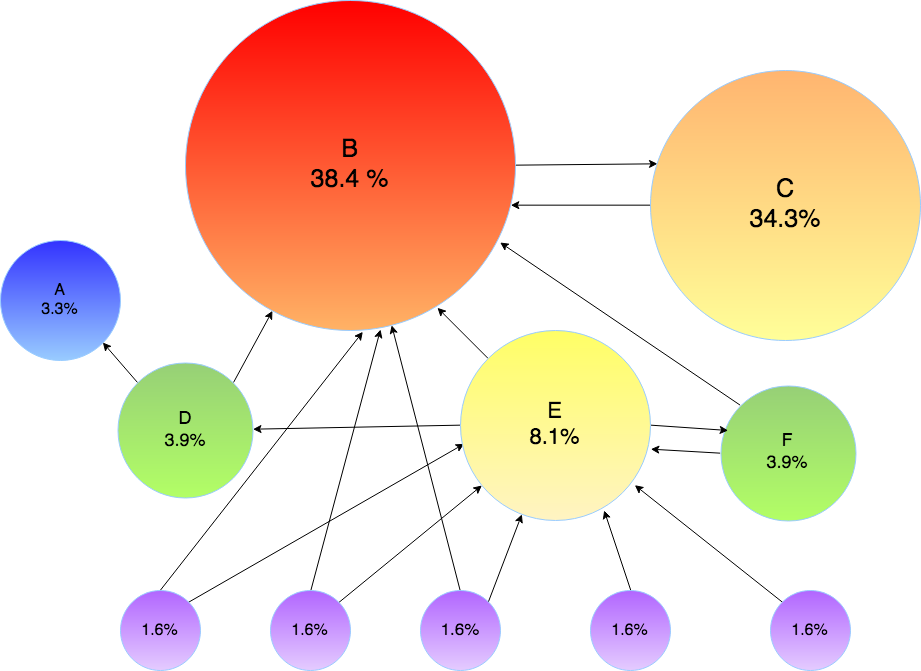
\includegraphics[height=6cm]{img/page_rank_example.png}
	\caption{PageRank example}
	\label{fig:prexample}
\end{figure}

As we can see in Fig ure \ref{fig:prexample}, node C has higher PageRank than A even if it has the same number of inner links; this is because the only inner link of C is from the most important node of the graph B so it is considered to be more important than the inner link of node A.

While surfing websites, going from one page to another I want to avoid problems with pages without outer links so I introduce two different methods to choose the next page. The surfer can:
\begin{itemize}
\item randomly choose an outgoing link from the page,
\item choose a random page from the network.
\end{itemize}
We assume that the surfer follows the first option with probability $p$ (typically $p=0.85$) and the second with probability $1-p$. This theoretical random walk is known as a Markov chain or Markov process.

The probability that an infinite random surfer visits a specific website is called its PageRank; a page will have high rank if other pages with high rank link to it.


\subsection{How to compute PageRank values}
To apply PageRank, from a graph of $n$ nodes we construct a $n$-by-$n$ connectivity matrix G such that
\begin{equation*}
g_{ij}=1 \text{\;\;\; if and only if nodes $i$ and $j$ are connected.} 
\end{equation*}
The number of non-zeros in $G$ is the total number of connections in the graph.

The row $r_i$ represents the number of inner-links of page $i$, while column $c_i$ the number of outer-links. So we can define:
\begin{itemize}
\item In-degree of page $i$: \tab $\:\:\:\:r_i = \sum\limits_{j=1}^{n} g_{ij}$
\item Out-degree of page $i$: \tab $c_i = \sum\limits_{j=1}^{n} g_{ji}$
\end{itemize}
Let $p$ be the probability that the surfer follows a link and $1-p$ the probability that it chooses a random page, then $\delta = \frac{1-p}{n}$ is the probability that a particular random page is chosen.

We construct a transition probability matrix A where all elements are positive, smaller than one and sums of columns are equal to one; column $j$ represents the probabilities to go from page j to all other pages. So we set
\begin{equation}\notag
a_{ij} = 
\begin{cases}
\frac{pg_{ij}}{c_{j}} + \delta  & \text{if } c_{j} \neq 0\\
\frac{1}{n} & \text{if } c_{j} = 0
\end{cases}
\end{equation}
In other words, if page $j$ has no outer links, it means that column $j$ of $A$ present a uniform probability $\frac{1}{n}$ in all its elements. Since matrix A is a transition matrix of a Markov chian, all its eigenvalues are real, between 0 and 1, and 1 is an eigenvalue itself. 

We can now compute PageRank values by solving the problem. 

\begin{equation}\notag
A\:x = x
\end{equation}

It is a particular eigenvalue problem because usually they are of the form $Ax=\lambda x$. Finding the solution of eigensystems is complicated and doesn't exist direct methods; the process has to be iterative such as the power or Jacobi methods.

In our specific problem we have $\lambda = 1$ so the power method seems to be the most effective. It computes the eigenvector relative to the greatest eigenvalue and it is our problem since A is a matrix of a Markov chain.

The transition matrix $A$ can be written as
$$A = pGD+ez^{T}, $$
where $D$ is a diagonal matrix with the reciprocals of the out-degrees, i.e.,
\begin{equation}\notag
d_{jj} = 
\begin{cases}
\frac{1}{n} & \text{if } c_{j} \neq 0\\
0 & \text{if } c_{j} = 0
\end{cases} \,,
\end{equation}
$z$ is the vector formed by
\begin{equation}\notag
z_{j} = 
\begin{cases}
\delta & \text{if } c_{j} \neq 0\\
\frac{1}{n} & \text{if } c_{j} = 0
\end{cases} \,,
\end{equation}
and e is the vector of length n with all ones.

We can write the linear system
$$(I-A)x=0$$
as
$$(I - pGD)x = \gamma e$$
where $\gamma = \transp{z}x$.
To conclude, since the value of the scalar $\gamma$ depends on the unknown $x$, we impose the condition $\gamma = 1$, then solve
\begin{equation}\notag
(I - pGD)x = e
\end{equation}
and then rescale the solution so that $\sum\limits_{i=1}^{n} x_i = 1$.

\begin{algorithm}
\caption{ (PageRank)}\label{pagerank}
\begin{algorithmic}[1]
\Procedure{PageRank}{}
\State $\textit{U} \gets \text{list of }\textit{authors}$
\State $\textit{G} \gets \text{adjacency matrix}$
\State $p \gets \text{dumping factor}$
\State $\textit{G} \gets \textit{G} - \text{diag(}\textit{G}\text{)} \: \: \: \text{(remove self collaborations)}$
\State $\textit{c} \gets \text{sum(}\textit{G}\text{,1)} \:\:\: \textit{r} \gets \text{sum(}\textit{G}\text{,2)} \:\:\: \text{(Compute out-degree and in-degree of each node)}$
\State $\textit{D} \gets \text{Diagonal matrix with reciprocals of out-degrees}$
\State $(I - pGD)x = e$
\State $x \gets x / sum(x) \: \:\: \text{(normalize the result x)}$
\State $x \gets \text{sort x in descending order}$\\
\Return x
\EndProcedure
\end{algorithmic}
\end{algorithm}






%%%%%%%%%%%%%%%%%%%%%%%%%
\section{The Graph Partitioning Algorithm} \label{sec:graphpart} 
%%%%%%%%%%%%%%%%%%%%%%%%%
Graph partitioning consists in dividing a graph $G=(V,E)$\footnote{A graph G with vertexes V and edges E.}  cutting the smaller number of edges and obtaining sub-graphs with specific properties. For example k-way partitioning divides the graph G into k smaller components.

A partitioning algorithm is said to be efficient if it divides a given graph into smaller components with about the same size, cutting as few edges as possible. 
A valid and fast method is the coordinate bisection, which simply chooses a partitioning plane perpendicular to one of the coordinate axes but spectral algorithm is more efficient. It finds a partition based on the eigenvalues and eigenvectors of the Laplacian matrix of the graph and doesn't need the nodal coordinates.

As we can see in Figure \ref{fig:partitioning} sometimes coordinate and spectral partitioning behave similarly but usually the second one is more effective.
\begin{figure}[ht]
	\centering
	\subfigure[]{
		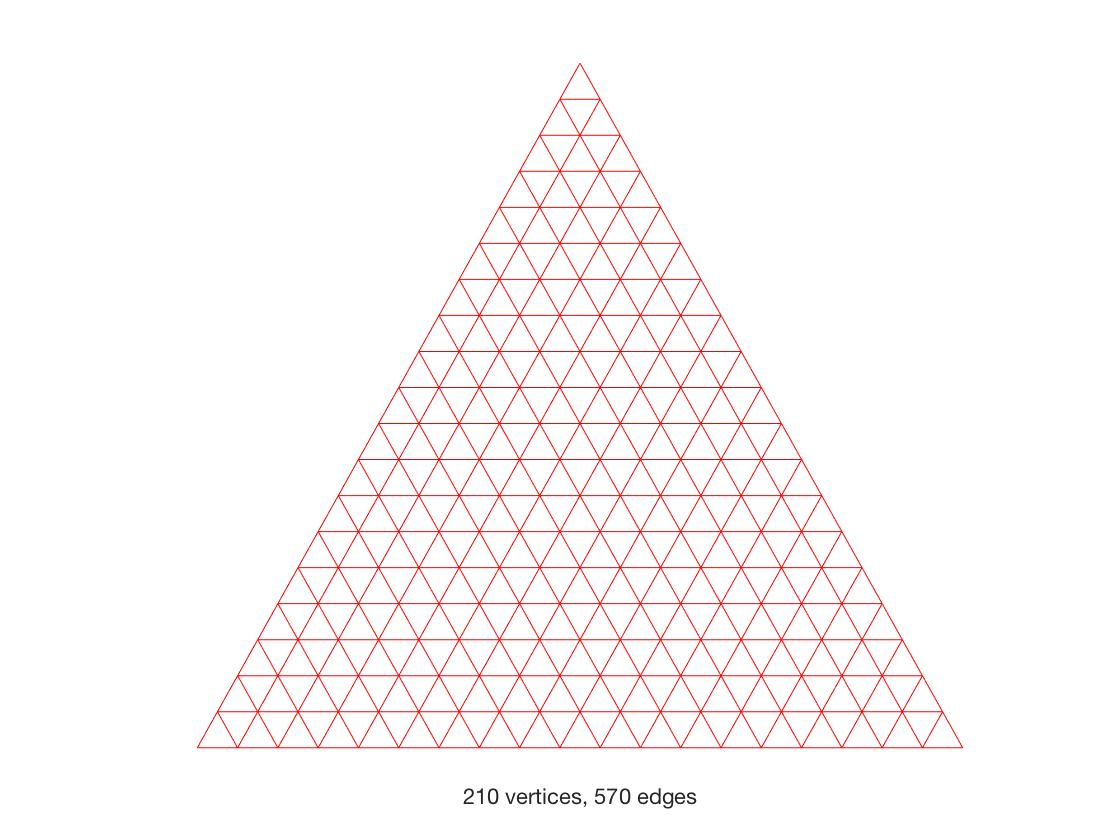
\includegraphics[height=4cm]{img/g4.jpg}
		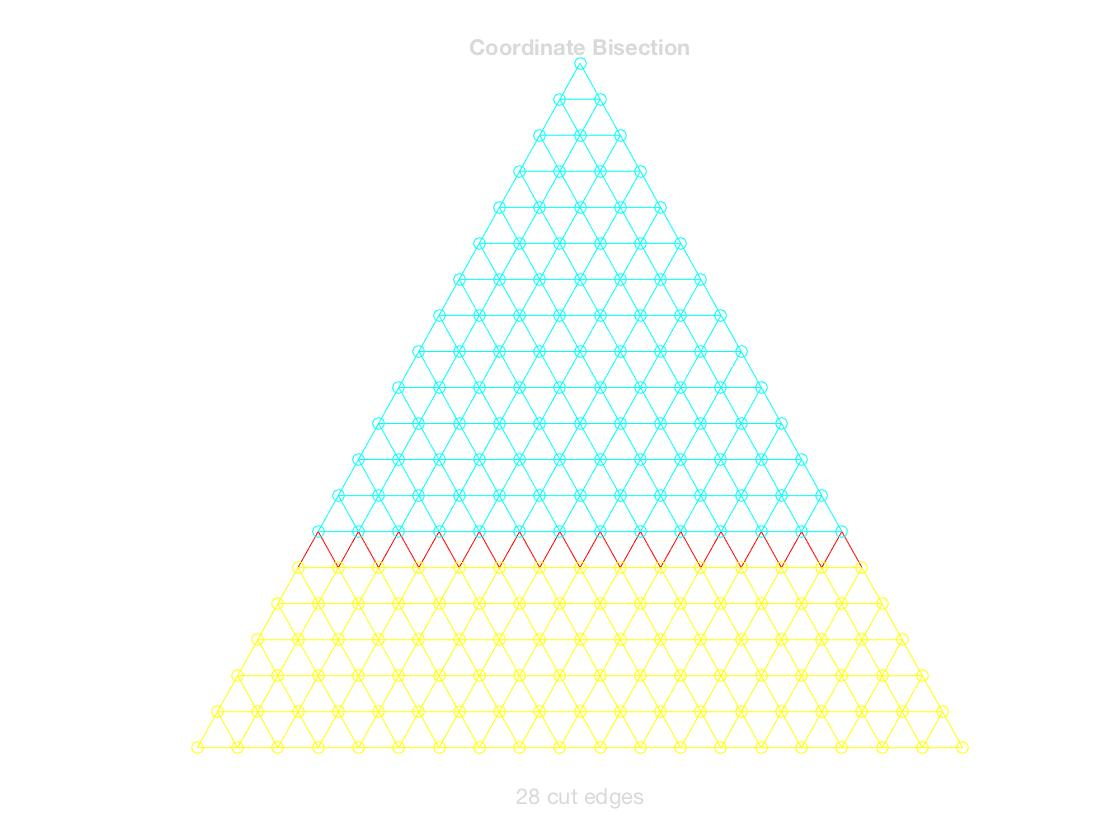
\includegraphics[height=4cm]{img/g5.jpg}
		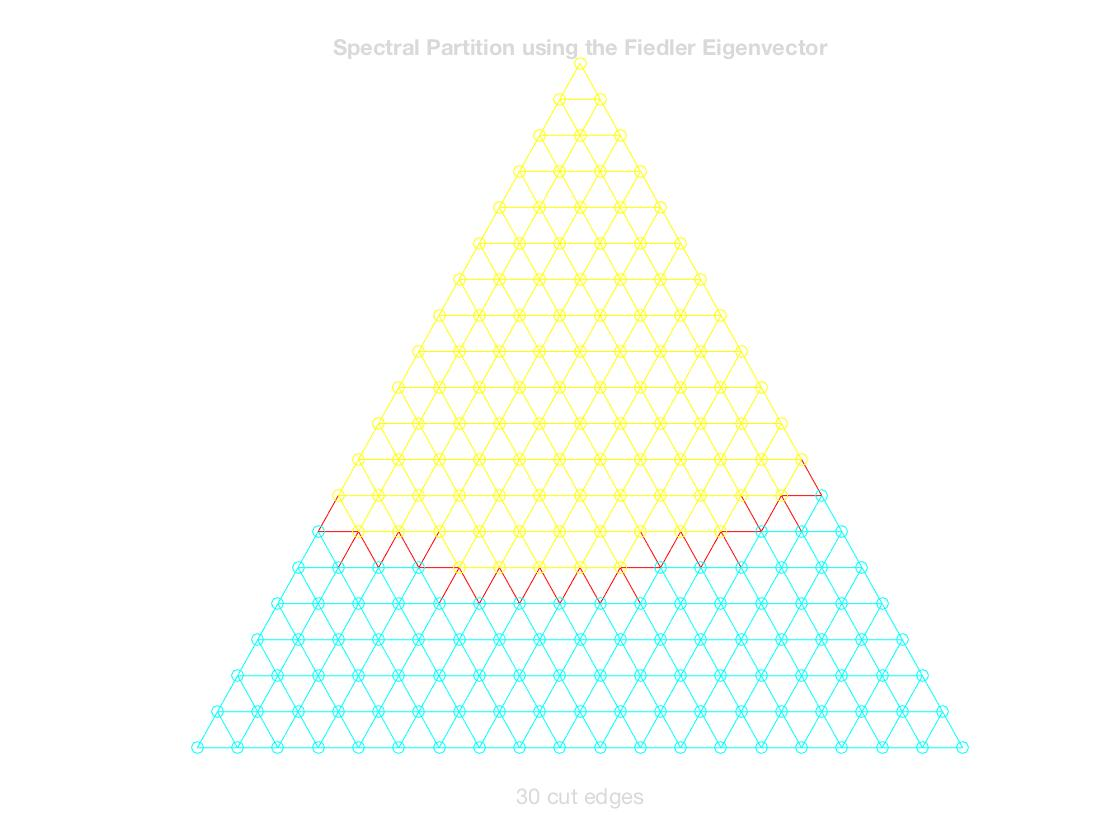
\includegraphics[height=4cm]{img/g6.jpg}
		\label{fig:corandsp}
	}
	\subfigure[]{
		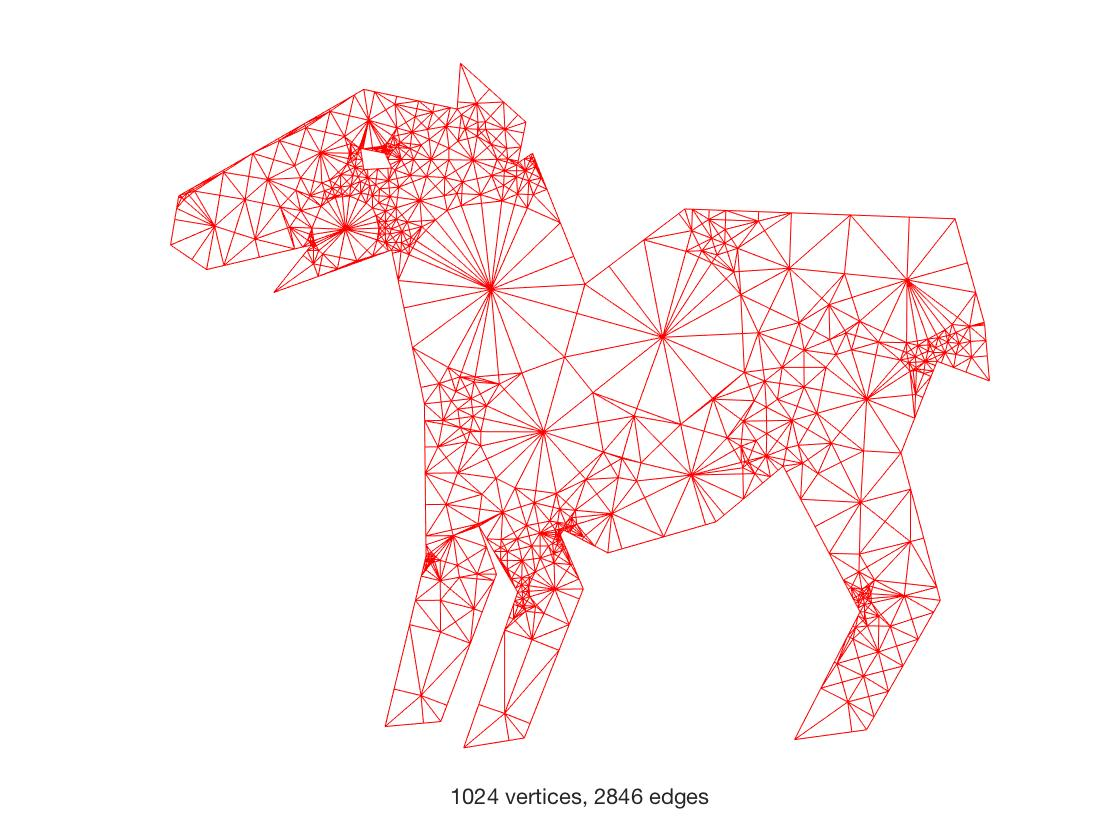
\includegraphics[height=4cm]{img/g10.jpg}
		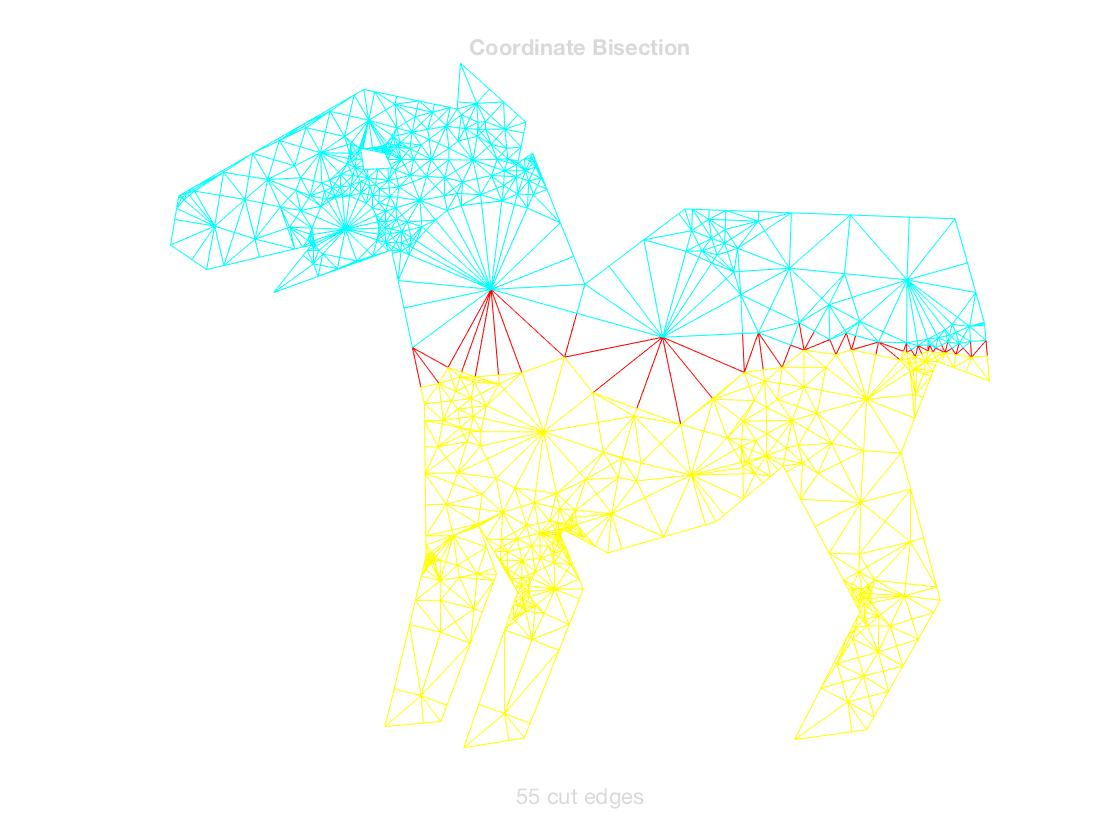
\includegraphics[height=4cm]{img/g11.jpg}
		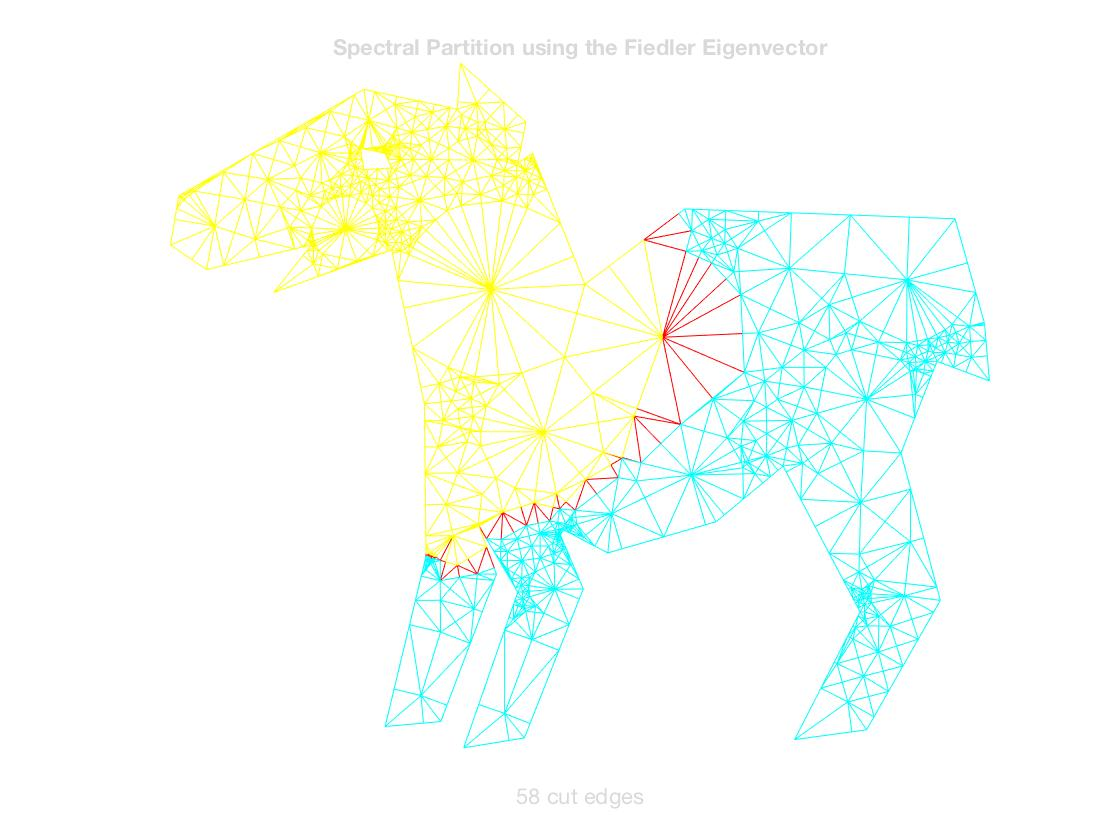
\includegraphics[height=4cm]{img/g12.jpg}
		\label{fig:cororsp}
	}
	\caption{In both \subref{fig:corandsp} and \subref{fig:cororsp} we have the graph at the left, the coordinate bisection in the middle and the spectral partition on the right}
	\label{fig:partitioning}
\end{figure}

\subsection{How to apply spectral graph partitioning}
To apply graph partitioning we need the adjacency matrix $A$ of the graph, which is symmetric since the graph is considered to be undirected, and the Laplacian matrix $L$ constructed such that: 
\begin{equation}\notag
L_{ij} = 
\begin{cases}
d_i \tab \:\:\: if \:\: i=j \\
-1 \tab if \:\: i \neq j \:\: and \: \: (i,j) \in E \\
0 \tab \:\:\:\: \text{otherwise}
\end{cases}
\end{equation}
where $d_i$ is the vertex degree of node $i \in V$.
The relation between A and L is
\begin{equation}\notag
L = D - A
\end{equation}
where D is the diagonal matrix having the $d_i$'s on the diagonal. Since L is symmetric and positive semidefinite by construction, all its eigenvalues are real and nonnegative. The first eigenvalue is always zero and, in the general case, the multiplicity of the the first eigenvalue corresponds to the number of connected components of the graph.

The eigenvalues of L are ordered as follows:
\begin{equation}\notag
0 = \lambda_1 = \ldots = \lambda_m < \lambda_{m+1} \le \ldots \lambda_n
\end{equation}

The eigenvector corresponding to the first eigenvalue $\lambda_1$ is the vector of all ones and it does not provide information about the graph structure; the second lowest eigenvector, instead, called ``Fiedler eigenvector'', is used by spectral partitioning to return the smaller sub-graphs. Dividing the nodes of graph G according to the median $s$ of the Fiedler vector $v = (v_1,v_2,...,v_n)$ gives two partitions $V_1$ and $V_2$ such that
\begin{equation}\notag
\begin{cases}
v_i \in V_1 \text{\;\; if \;\;} v_i \leq s \\
v_i \in V_2 \text{\;\; if \;\;} v_i > s
\end{cases} .
\end{equation}
Such a partition is called the Fiedler cut and leads to two parts of G with nearly equal number of vertexes, minimizing the number of cut edges. 

Fiedler theorem said that if the graph G is connected, L the Laplacian matrix, $N_+$ and $N_-$ a partitioning such that
\begin{equation}\notag
x(i) = +1 \tab \text{if } v_i \text{in } N_+ 
\end{equation}
\begin{equation}\notag
x(i) = -1 \tab \text{if } v_i \text{in } N_-
\end{equation}

Then the number of edges cut is:
\begin{equation}\notag
\#\text{edge\_cut} = \frac{1}{4}x^T L x
\end{equation}

This problem of minimizing the number of cut edges is NP-hard and can be written as a constrained minimization problem:
\begin{equation}\notag
\min\limits_z f(z)=\frac{1}{4} z^T L z \tab \text{subject to} \tab 
\begin{cases}
z^T z = n \tab \text{z is a real vector}\\
z^T e = 0 \tab \text{with } e=[1,1,...,1]^T
\end{cases}
\end{equation}


\begin{algorithm}
\caption{ (Graph Partitioning)}\label{gpartitioning}
\begin{algorithmic}[1]
\Procedure{Graph Partitioning}{}
\State $\textit{G} \gets \text{(V,E)}$
\State $\text{compute Fiedler vector of } \textit{L = D - A}$
\State $\text{Sort the vector values}$
\State $\text{Put first half of the nodes in } V_1 \text{ and second half in } V_2$
\State $ E_1 \gets \text{ edges with both nodes in } V_1$
\State $ E_2 \gets \text{ edges with both nodes in } V_2$\\
\Return $\textit{G1} = \text{(V1,E1) and } \textit{G2} = \text{(V2,E2)}$
\EndProcedure
\end{algorithmic}
\end{algorithm}



\subsection{K-way Partitioning}
K-way partitioning of a graph G of n nodes, consists in a division of its nodes in k disjoint subset, all with size nearly $\frac{n}{k}$ (see Figure \ref{fig:kpartitioning}).

\begin{figure}[ht]
	\centering
	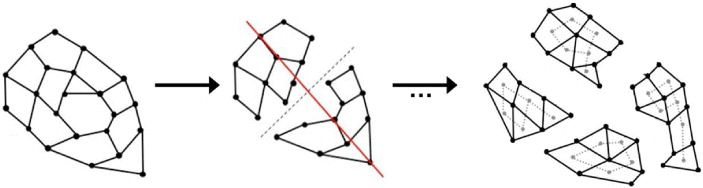
\includegraphics[height=3cm]{img/k_way_partitioning.jpg}
	\caption{Example of k-way graph partitioning}
	\label{fig:kpartitioning}
\end{figure}

We consider only the simple case where we want to divide the graph in k partitions and k is a power of two. The idea is just to apply the spectral partitioning $\frac{k}{2}$ times recursively to each of the partitions obtained. The method is presented in Algorithm~\ref{kpartitioning}.

\begin{algorithm}
\caption{ (k-way Partitioning)}\label{kpartitioning}
\begin{algorithmic}[1]
\Procedure{k-way Partitioning}{}
\State $\textit{G} \gets \text{(V,E)}$
\State $k \gets \text{number of desired partitions}$
\State $\text{Apply spectral partitioning on G and find }G_1 \text{ and } G_2$
\BState \emph{loop}:
\If {$\frac{k}{2} > 1$}
\State $\text{Recursive partition on }G_1 \text{ with } \frac{k}{2}$
\State $\text{Recursive partition on }G_2 \text{ with } \frac{k}{2}$
\State $k \gets \frac{k}{2}$
\EndIf
\State \textbf{goto} \emph{loop}\\
\Return $G_1 = (V_1,E_1) \text{ ... } G_K = (V_K,E_K)$
\EndProcedure
\end{algorithmic}
\end{algorithm}


\section{Numerical analysis}
After retrieving all the necessary information and organizing the data in adjacency matrix, I applied PageRank and Graph Partitioning algorithms, obtaining the following results.
Since the Swiss authors' names obtained are only 422, I decide to extend the research to the institutions from all over the word, reaching 16425 names. 

I first construct the adjacency matrix of the authors and their corresponding universities; for the universities I also build a weighted matrix which keep the number of collaborations between each university. We can see the matrices obtained in figure \ref{fig:authorsAdj} and \ref{fig:univAdj}

\begin{figure}[ht]
	\centering
	\subfigure[]{
		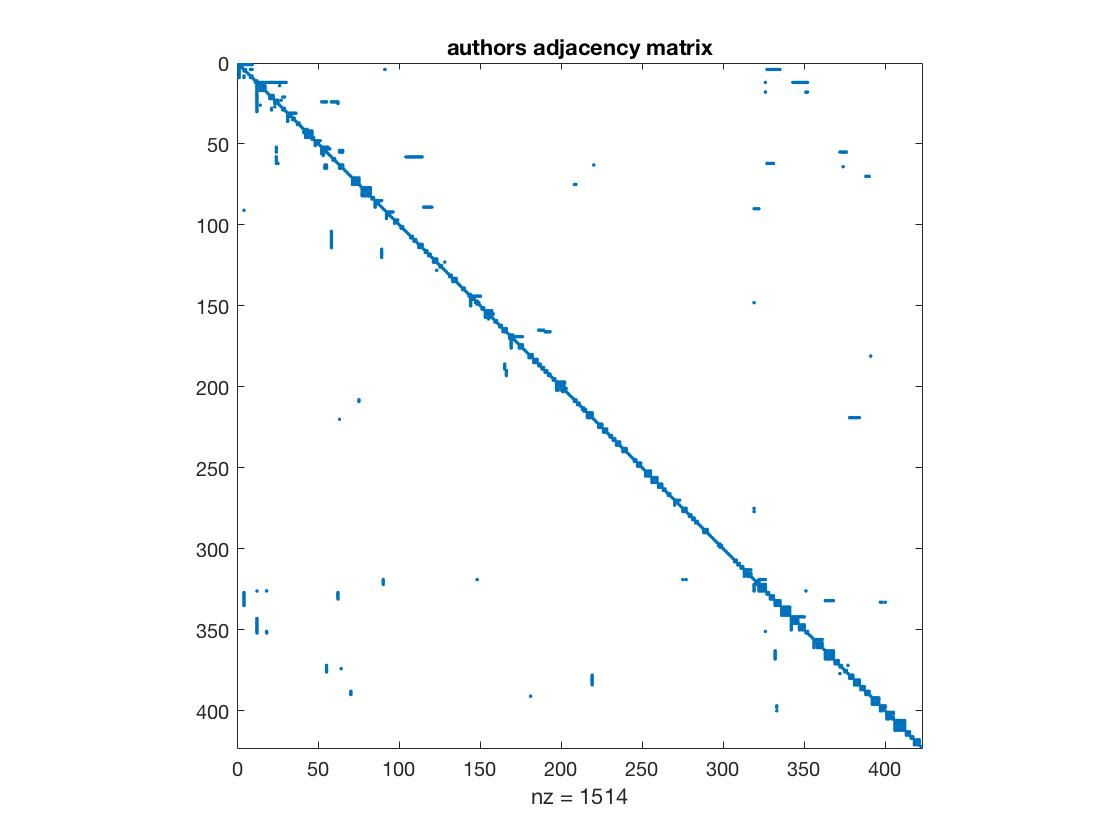
\includegraphics[height=5cm]{img/Analysis/authors_adj.jpg}
		\label{fig:AdjS}
	}
	\subfigure[]{
		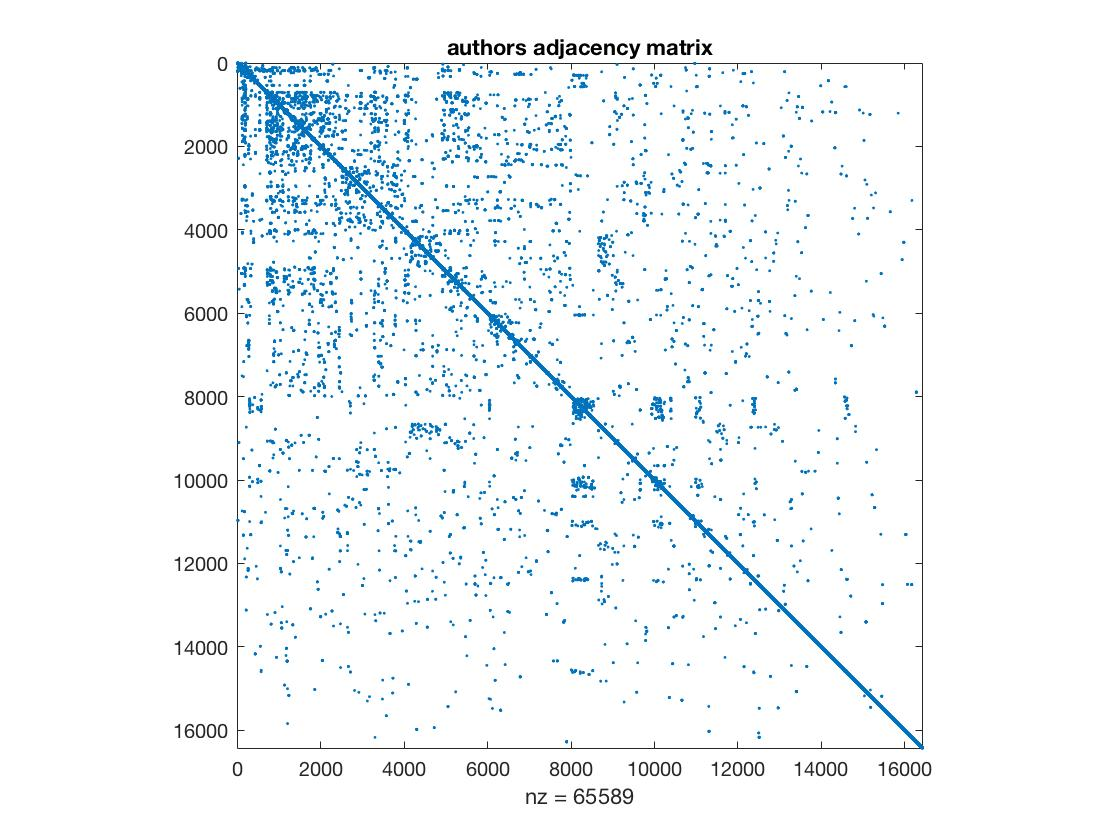
\includegraphics[height=5cm]{img/Analysis_world/author_adj.jpg}
		\label{fig:AdjW}
	}
	\caption{\subref{fig:AdjS} is the Swiss authors' adjacency matrix and \subref{fig:AdjW} is the one of the world authors}
	\label{fig:authorsAdj}
\end{figure}

\begin{figure}[ht]
	\centering
	\subfigure[]{
		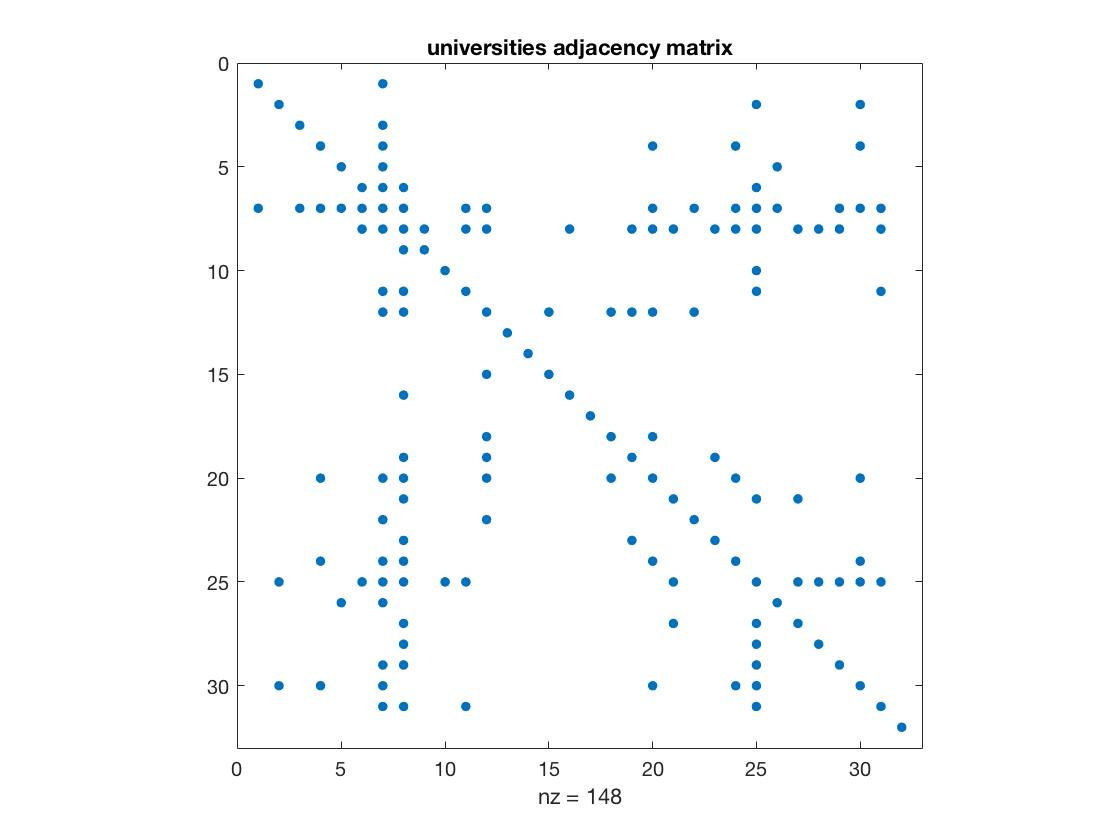
\includegraphics[height=5cm]{img/Analysis/univ_adj.jpg}
		\label{fig:uniAdj}
	}
	\subfigure[]{
		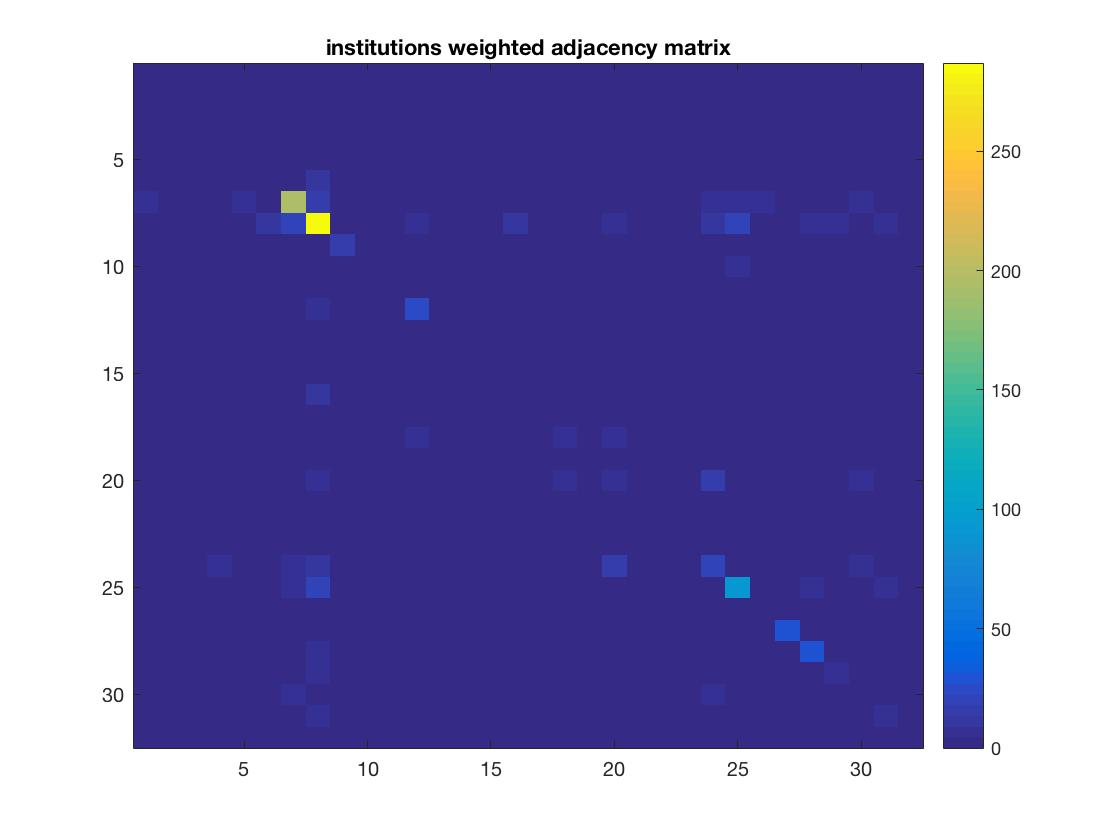
\includegraphics[height=5cm]{img/Analysis/univ_adj_weighted.jpg}
		\label{fig:uniAdjW}
	}
	\caption{ \subref{fig:uniAdj} is the Swiss university adjacency matrix, \subref{fig:uniAdjW} is the universities weighted graph}
	\label{fig:univAdj}
\end{figure}

The sparsity of the Swiss author adjacency matrix is $0.0085$ instead the one of world author matrix is $2.4312*10^{-04}$.

The universities that collaborate more in Switzerland are the École polytechnique fédérale de Lausanne and the ETH Zürich which correspond to the indexes 7 and 8 in the matrix. In the weighted matrix we can observe that these two universities collaborate both internally in the university but also with other institutions: for example  ETH Zürich has 19 collaboration with Università della Svizzera italiana.


\subsection{PageRank -- forse (inclusi in R.analysis)}
\begin{figure}[ht]
	\centering
	\subfigure[]{
		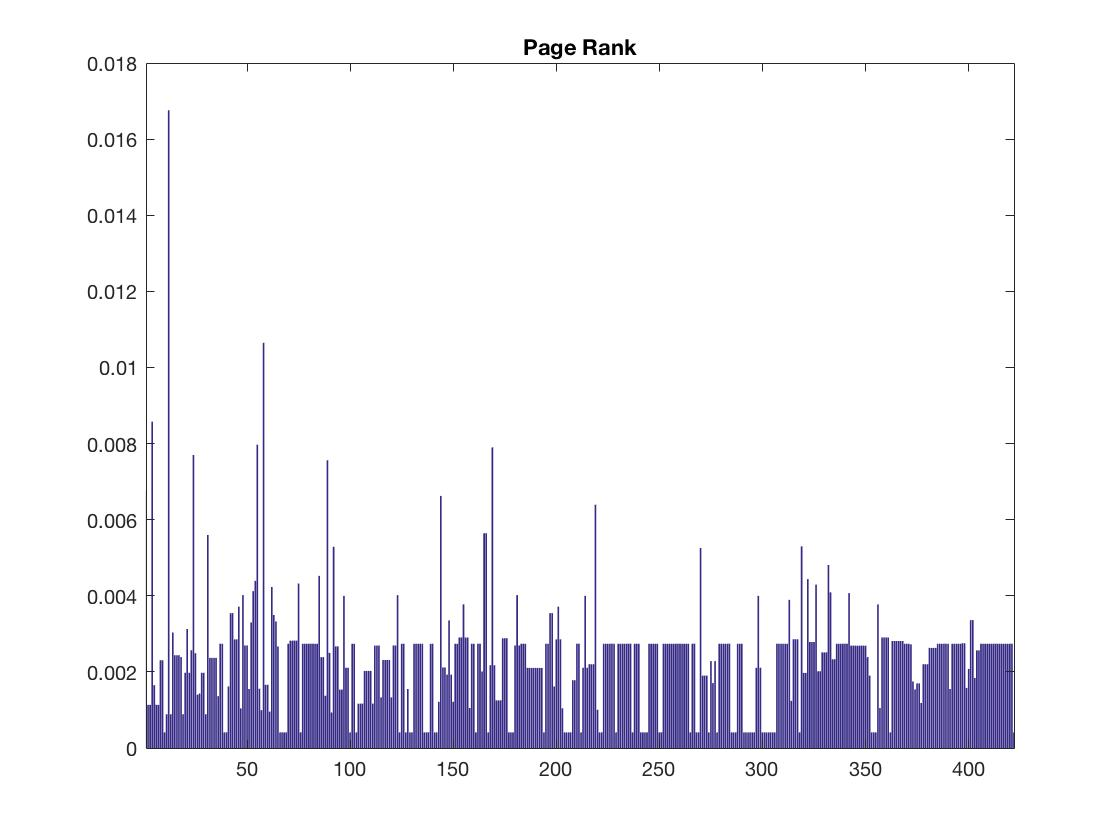
\includegraphics[height=6cm]{img/Analysis/page_rank_bars.jpg}
		\label{fig:PRbars}
	}
	\subfigure[]{
		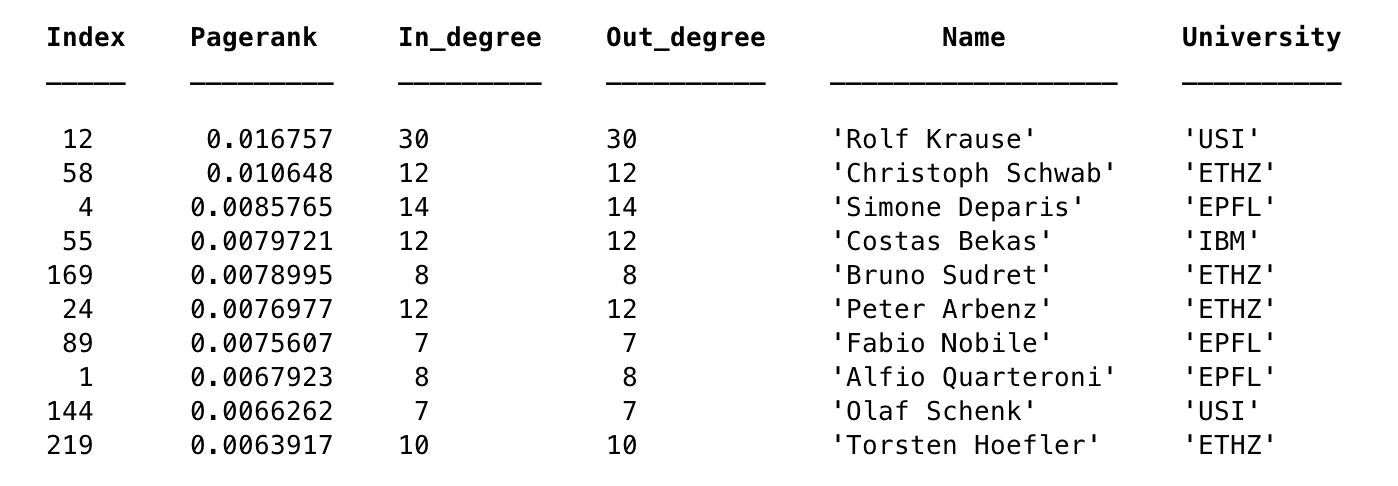
\includegraphics[height=4.5cm]{img/Analysis/Pagerank_swiss_10}
		\label{fig:PRlist}
	}
	\caption{ \subref{fig:PRbars} is a bar graph of PageRank values, \subref{fig:PRlist} are the first 15 people with higher PageRank value}
	\label{fig:PRAuthors}
\end{figure}

\begin{figure}[ht]
	\centering
	\subfigure[]{
		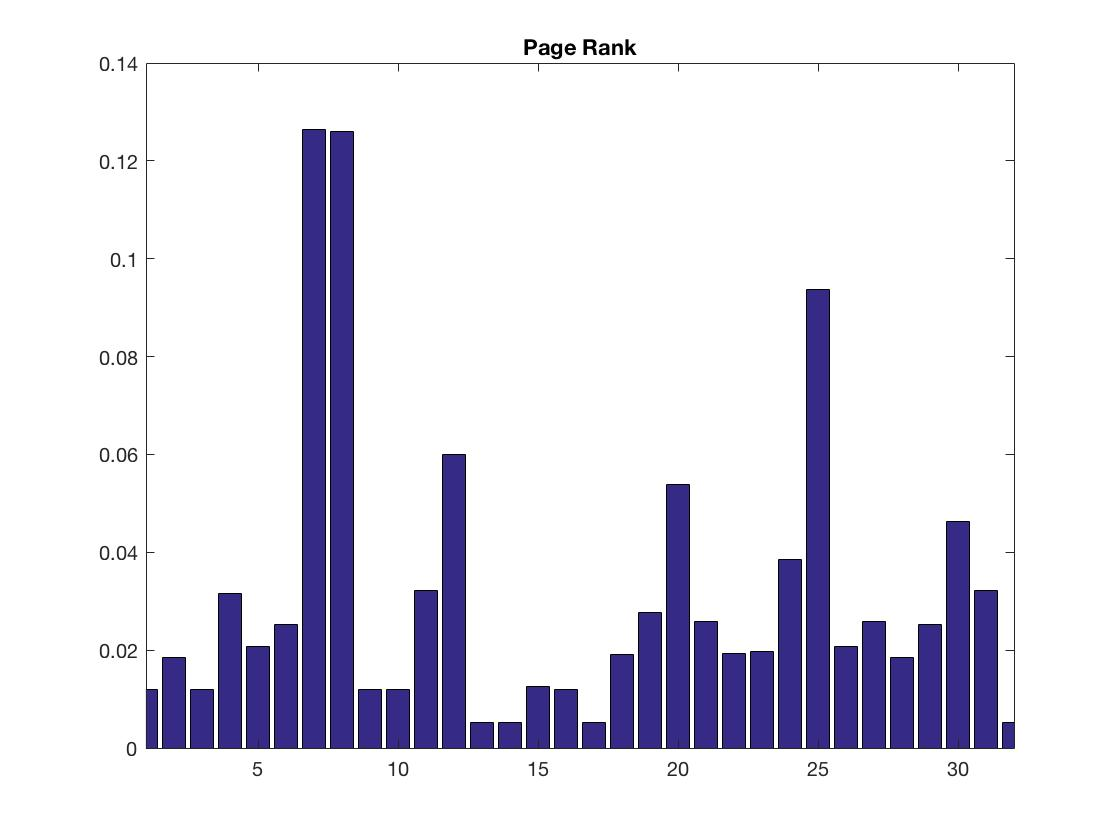
\includegraphics[height=6cm]{img/Analysis/page_rank_uni.jpg}
		\label{fig:PRbarsuni}
	}
	\subfigure[]{
		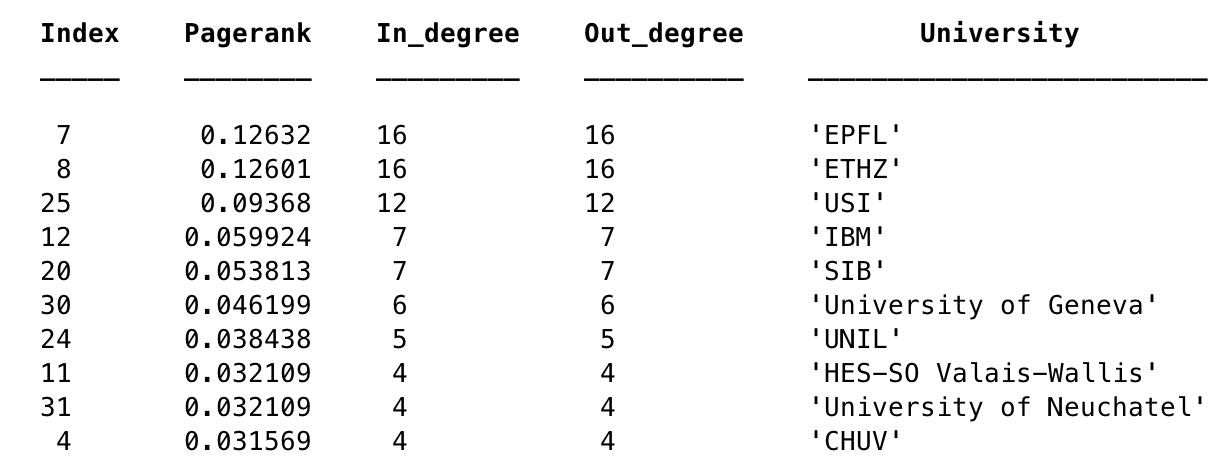
\includegraphics[height=4.5cm]{img/Analysis/pr_uni_10}
		\label{fig:PRlistuni}
	}
	\caption{ \subref{fig:PRbars} is a bar graph of PageRank values, \subref{fig:PRlist} are the first 15 universities with higher PageRank value}
	\label{fig:PRUniversities}
\end{figure}
\subsection{Graph Partitioning -- forse (inclusi in R.analysis)}

\begin{figure}[ht]
	\centering
	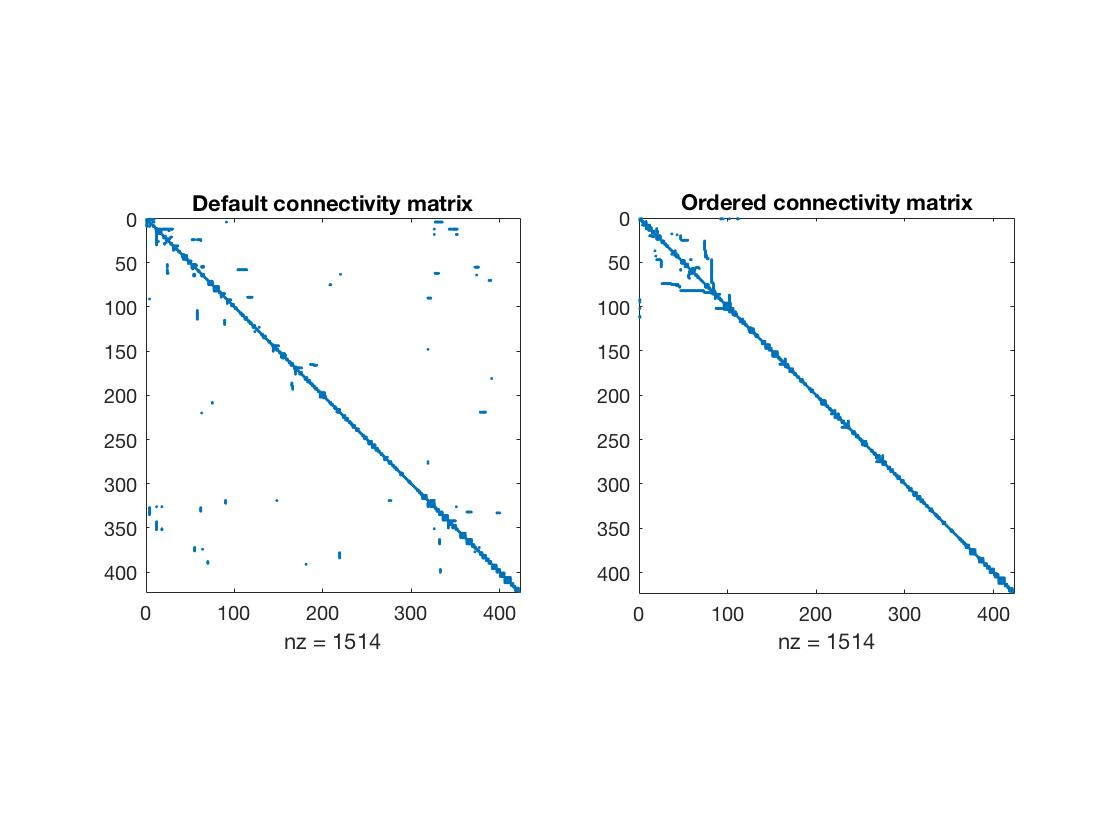
\includegraphics[height=6cm]{img/Analysis/cuthill_mckee.jpg}
	\caption{The Reverse Cuthill McKee ordering}
	\label{fig:CuthillMcKee}
\end{figure}

\begin{figure}[ht]
	\centering
	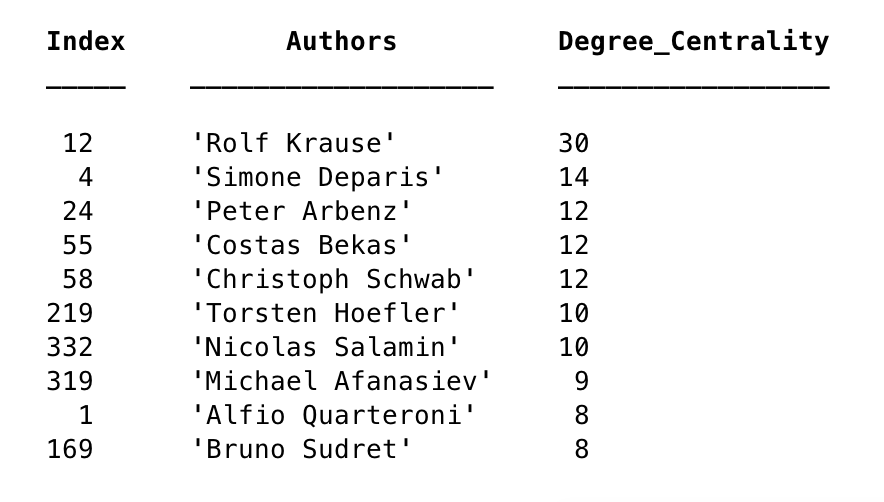
\includegraphics[height=5cm]{img/Analysis/degree_centrality}
	\caption{Degree Centrality}
	\label{fig:degree}
\end{figure}

\begin{figure}[ht]
	\centering
	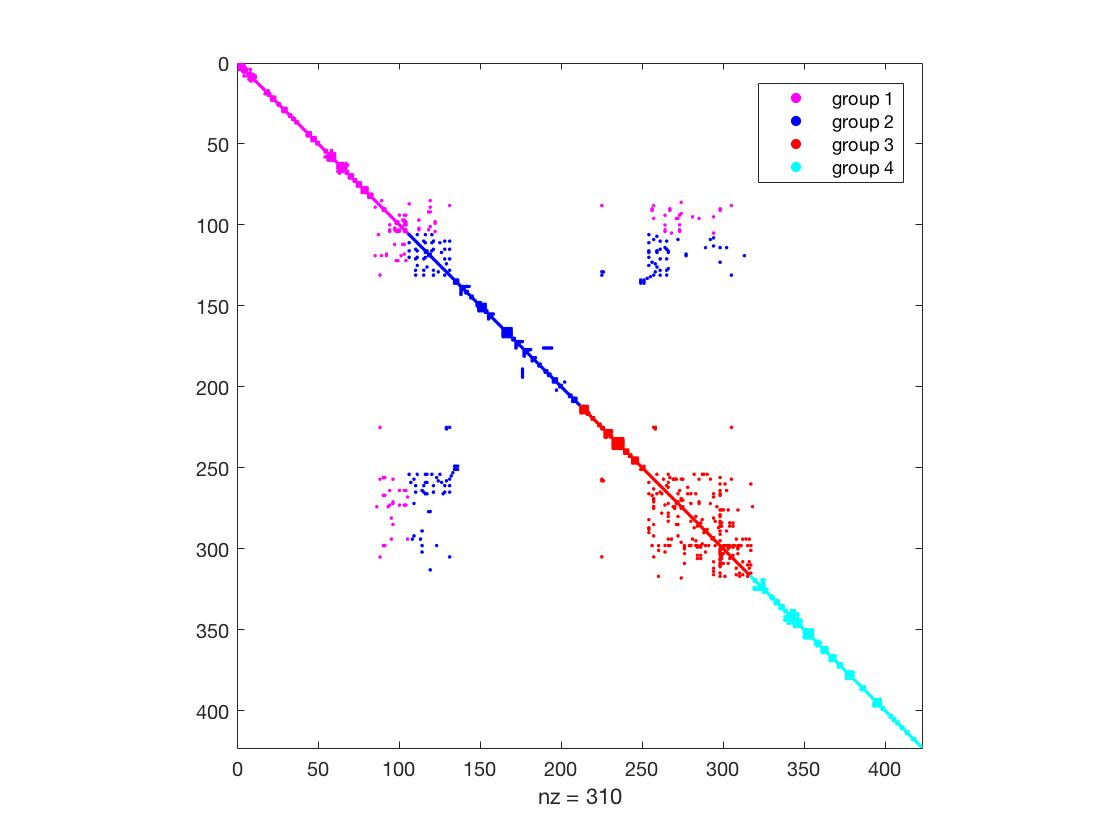
\includegraphics[height=6cm]{img/Analysis/graph_partitioning.jpg}
	\caption{The graph partitioning algortihm}
	\label{fig:graphPart}
\end{figure}


\newpage
\section{Bibliography  \textcolor{red}{Temporary}}
\begin{itemize}
\item https://en.wikipedia.org/wiki/PageRank
\item Assignment1 1 Course Numerical Computing 2107/2018
\item Assignment2 1 Course Numerical Computing 2107/2018
\item \hyperref[label_name]{''https://am.vsb.cz/export/sites/am/cs/theses/kabelikova\_ing.pdf''}
\item https://en.wikipedia.org/wiki/Graph\_partition
\end{itemize}





% Footnotes
%Cliques\footnote{Some text in a footnote.} \ldots


%Immagini
%\begin{figure}[ht]
%	\centering
%	\subfigure[]{
%		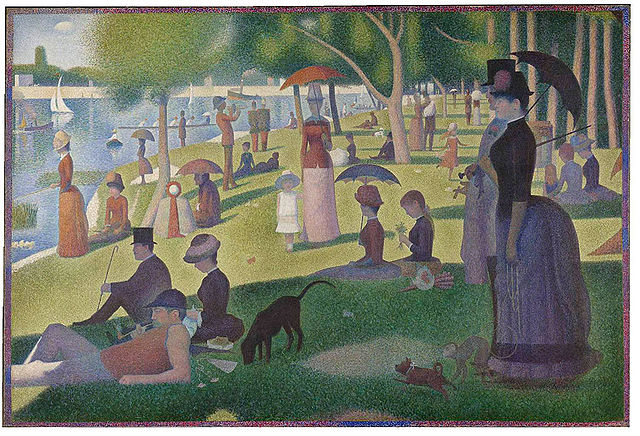
\includegraphics[height=6cm]{img/seurat.jpeg}
%		\label{fig:seurat}
%	}
%	\subfigure[]{
%		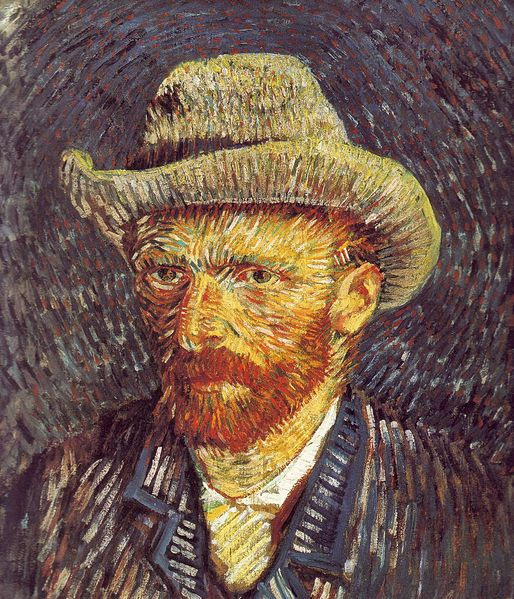
\includegraphics[height=6cm]{img/gogh.jpeg}
%		\label{fig:gogh}
%	}
%	\caption{Famous examples of divisionism painting: \subref{fig:seurat} ``Un dimanche apr\`es-midi \`a l'\^Ile de la Grande Jatte'' (1884-1886) by Georges Seurat and \subref{fig:gogh} ``Self Portrait with felt Hat'' (1887-1888) by Vincent van Gogh.}
%	\label{fig:divisionism}
%\end{figure}


%Referenza a immagini
% whose greatest exponent was Georges Seurat (see Figure \ref{fig:seurat}).
 
 
% Referenza bibliografica
%In this project I implemented an algorithm for extracting a resolution-independent vector representation from pixel art images, based on the paper of Johannes Kopf and Dani Lischinski \cite{Kopf2011}. 


% algorithm
%\begin{algorithm}
%\caption{ (PageRank algorithm)}\label{pagerank}
%\begin{algorithmic}[1]
%\Procedure{MyProcedure}{}
%\State $\textit{U} \gets \text{list of }\textit{authors}$
%\State $\textit{G} \gets \text{adjacency matrix}$
%\State $p \gets \text{dumping factor}$
%\BState \emph{top}:
%\If {$i > \textit{stringlen}$} \Return false
%\EndIf
%\State $j \gets \textit{patlen}$
%\BState \emph{loop}:
%\If {$\textit{string}(i) = \textit{path}(j)$}
%\State $j \gets j-1$.
%\State $i \gets i-1$.
%\State \textbf{goto} \emph{loop}.
%\State \textbf{close};
%\EndIf
%\State $i \gets i+\max(\textit{delta}_1(\textit{string}(i)),\textit{delta}_2(j))$.
%\State \textbf{goto} \emph{top}.
%\EndProcedure
%\end{algorithmic}
%\end{algorithm}


%\newpage
%%%%%%%%%%%%%%%%%%%%%%%%%%
%\section{Conclusions} \label{sec:conclusions}
%%%%%%%%%%%%%%%%%%%%%%%%%%
%
%I have implemented an algorithm for extracting a resolution-independent vector representation from pixel art images. This algorithm resolves separation/connectedness ambiguities in the square pixel lattice and then reshapes the pixel cells so that both cardinal and diagonal neighbors of a pixel are connected through edges. The regions with smoothly varying shading are extracted and separated through piecewise smooth contour curves. I have demonstrated that conventional image upsampling and vectorization algorithms cannot handle pixel art images well, while this algorithm produces good results on a wide variety of inputs.
%
%
%\subsection{Future work} \label{sec:future}
%
%There are many possibilities for future work. The implementation still suffers from some limitations (Section \ref{sec:limitations}) which could be corrected or improved, but also more features can be added to increase the number of different applications for this algorithm.
%
%
%\subsection{Acknowledgments}
%
%I want to thank my project advisor, prof. Kai Hormann, for suggesting this fascinating project. I really enjoyed working on it and prof. Hormann has been very helpful throughout the whole project. I was given a lot of freedom and independence, which pushed me to give the best of myself. The project had such a great potential and was so intellectually challenging that I was thrilled and eager every time I could spend time working on it.\\
%I also want to thank my wife for being so supportive and patient. The long nights passed working on this project really proved her love, and her caring for my well-being helped me a lot through the difficult and stressing moments. Her excitement for every new feature pushed me to improve the project more and more, seeking that wonderful smile.
%
%%%%%%
%\bibliographystyle{abbrv}
%\bibliography{references}

\end{document}